% gallery-title: Reachable
% gallery-category: Quantum 
% gallery-tags: model reduction
% gallery-description: 
% gallery-order: 10
% paper: arXiv:2412.05102

\documentclass{standalone}

\usepackage{siunitx}

\usepackage{amsfonts,amsmath,amssymb}
\usepackage{cancel}
\usepackage{amsfonts,amsmath,amssymb}
\usepackage[english]{babel}
\usepackage[normalem]{ulem}
\usepackage{hyperref}
\usepackage{amsthm}
\usepackage{graphicx}
\usepackage{xfrac}
\usepackage{subcaption,caption}
\usepackage{epsfig}
\usepackage{ulem}
\usepackage{tikz}
\usepackage{mathrsfs}
\usepackage{bbold}  
\usepackage{soul}
\definecolor{green}{RGB}{90, 190, 105} 
\usepackage{pgfplots}
\usepackage{pgfplotstable} 
\usepgfplotslibrary{groupplots}
\pgfplotsset{compat = newest}

\usepackage{bm}
\usetikzlibrary{shapes,arrows}
\usetikzlibrary{matrix}
\usetikzlibrary{3d}
\usetikzlibrary{calc,patterns,angles,quotes,arrows,automata}
\graphicspath{ {./imgs/}}
\usepackage{tikz-3dplot}

\usepackage{csvsimple}

% ---------------------- Calligrapic
\newcommand{\Ac}{\mathcal{A}}
\newcommand{\Bc}{\mathcal{B}}
\newcommand{\Cc}{\mathcal{C}}
\newcommand{\Dc}{\mathcal{D}}
\newcommand{\Ec}{\mathcal{E}}
\newcommand{\Gc}{\mathcal{G}}
\newcommand{\Oc}{\mathcal{O}}
\newcommand{\Hc}{\mathcal{H}}
\newcommand{\Jc}{\mathcal{J}}
\newcommand{\Rc}{\mathcal{R}}
\newcommand{\Mc}{\mathcal{M}}
\newcommand{\Sc}{\mathcal{S}}
\newcommand{\Pc}{\mathcal{P}}
\newcommand{\Zc}{\mathcal{Z}}
\newcommand{\Qc}{\mathcal{Q}}
\newcommand{\Ic}{\mathcal{I}}
\newcommand{\Kc}{\mathcal{K}}
\newcommand{\Lc}{\mathcal{L}}
\newcommand{\Tc}{\mathcal{T}}

% -------------------------- Script
\newcommand{\As}{\mathscr{A}}
\newcommand{\Bs}{\mathscr{B}}
\newcommand{\Cs}{\mathscr{C}}
\newcommand{\Ds}{\mathscr{D}}
\newcommand{\Ls}{\mathscr{L}}
\newcommand{\Os}{\mathscr{O}}
\newcommand{\Ss}{\mathscr{S}}
\newcommand{\Ns}{\mathscr{N}}
\newcommand{\Vs}{\mathscr{V}}
\newcommand{\Ws}{\mathscr{W}}
\newcommand{\Xs}{\mathscr{X}}
\newcommand{\Ys}{\mathscr{Y}}
\newcommand{\Zs}{\mathscr{Z}}

\newcommand{\Rs}{\mathscr{R}}
\newcommand{\Es}{\mathscr{E}}
\newcommand{\Ts}{\mathscr{T}}
\newcommand{\Us}{\mathscr{U}}
\newcommand{\Gs}{\mathscr{G}}
\newcommand{\Fs}{\mathscr{F}}

% -------------------------- Bold
\newcommand{\Rb}{\mathbb{R}}
\newcommand{\Nb}{\mathbb{N}}
\newcommand{\Cb}{\mathbb{C}}
\newcommand{\Pb}{\mathbb{P}}
\newcommand{\Eb}{\mathbb{E}}
\newcommand{\Jb}{\mathbb{J}}

% ------------------------- Fraktur
\newcommand{\Bf}{\mathfrak{B}}
\newcommand{\Ff}{\mathfrak{F}}
\newcommand{\Hf}{\mathfrak{H}}
\newcommand{\Df}{\mathfrak{D}}
\newcommand{\Gf}{\mathfrak{G}}
\newcommand{\Sf}{\mathfrak{S}}
\newcommand{\Zf}{\mathfrak{Z}}
\newcommand{\Pf}{\mathfrak{P}}
\newcommand{\Kf}{\mathfrak{K}}


% -------------------------- Conditional expectations etc
\newcommand{\CE}{\mathbb{E}|}
\newcommand{\SR}{\mathbb{S}|}
\newcommand{\SE}{\mathbb{J}|}

\newcommand{\cov}{{\mathbb{Cov}}}
\newcommand{\var}{{\mathbb{Var}}}

% -------------------------- Reduced operators 
\newcommand{\ro}{\mathcal{R}_0}
\newcommand{\eo}{\mathcal{J}_0}
\newcommand{\rs}{\mathcal{R}}
\newcommand{\es}{\mathcal{J}}

% ------------------------ Numbers
\newcommand{\um}{\frac{1}{2}}
\newcommand{\one}{\mathbb{1}}
\newcommand{\zero}{\mathbb{0}}

\newcommand{\onev}{{\bm 1}}
\newcommand{\zerov}{{\bm 0}}

% ----------------------- Functions and operations
\newcommand{\im}{{\rm Im}}
\newcommand{\id}{{\rm Id}}
\newcommand{\fix}{{\rm fix}}
\newcommand{\ad}{{\rm ad}}
\newcommand{\bin}{{\rm bin}}
\newcommand{\tr}{{\rm tr}}
\newcommand{\diag}{{\rm diag}}
\newcommand{\Span}{{\rm span}}
\newcommand{\cl}{{\rm cl}}
\newcommand{\spec}{{\rm spec}}
\newcommand{\idem}{ {\rm idem}}
\newcommand{\res}{{\rm res}}
\newcommand{\supp}{{\rm supp}}
\newcommand{\lind}{\mathcal{L}}
\newcommand{\alg}{{\rm alg}}
\newcommand{\img}{{\rm Im}}

\DeclareMathOperator{\rank}{rank}

\newcommand{\comp}{{\sim}}
\newcommand{\zentrum}{\mathcal{Z}}


% -------------------------- Inner products and co
\newcommand{\ket}[1]{\left| #1 \right>}
\newcommand{\bra}[1]{\left< #1 \right|}
\newcommand{\norm}[1]{\left|\left| #1 \right|\right|}
\newcommand{\inner}[2]{\left< #1,#2 \right>}
\newcommand{\Outer}[2]{ \left|#1\right>\left<#2\right| }
\newcommand{\expect}[1]{\left< #1 \right>}
\newcommand{\braket}[2]{\left< #1 \middle\vert #2 \right>}
\newcommand{\ketbra}[2]{\left\vert #1 \middle>\middle< #2 \right\vert}
\newcommand{\virg}[1]{\lq\lq{} #1\ignorespacesafterend\rq\rq}

% \usepackage{mathabx}
% \renewcommand{\check}{\widecheck}
% \renewcommand{\bar}{\overline}
% \renewcommand{\Tilde}{\widetilde}
% \renewcommand{\Hat}{\widehat}



% ------------------------ Comments
\newcommand{\blue}[1]{{\color{blue} #1}}
\newcommand{\red}[1]{{\color{red} #1}}
\newcommand{\green}{\color{teal}}

\definecolor{darkviolet}{rgb}{0.58, 0.0, 0.83}
\definecolor{lavender}{rgb}{0.45, 0.31, 0.59}

\newcommand{\TG}[1]{{\color{OrangeRed}#1}}

\newcommand{\LV}[1]{{\color{cyan}#1}}
%{{\color{darkviolet}#1}}
\newcommand{\VL}[1]{{\color{blue}#1}}

\newcommand{\FT}[1]{{\color{ForestGreen}#1}}
\newcommand{\DT}[1]{{\color{Mulberry}#1}}


\begin{document}

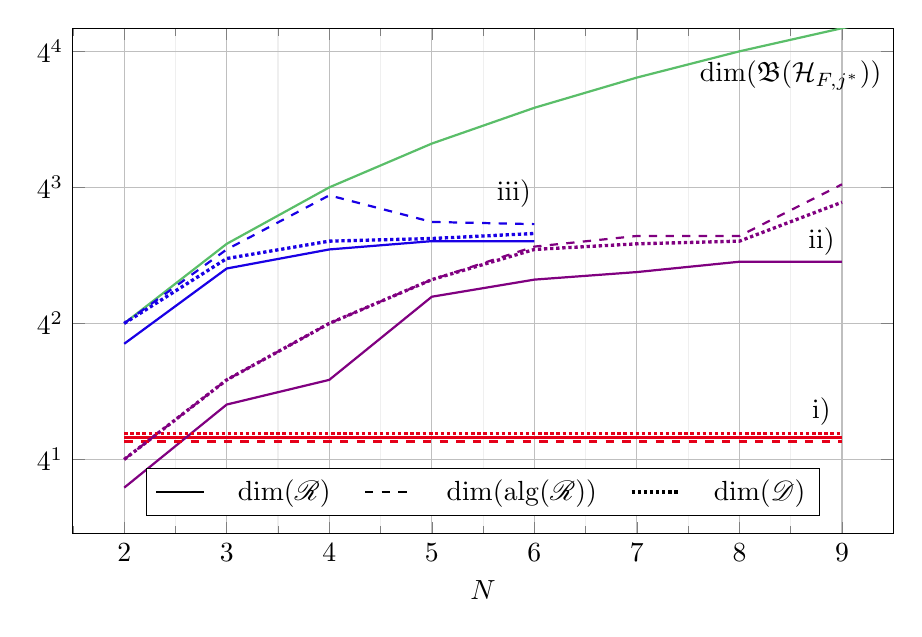
\begin{tikzpicture}

\begin{axis}[
xtick distance=1,
ymode=log,
grid = both,
xmin = 1.5, xmax = 9.5,
ymin = , ymax = 324,
xtick distance = 1,
ytick distance = 4,
grid = both,
minor tick num = 1,
major grid style = {lightgray},
minor grid style = {lightgray!25},
width = 12cm,
height = 8cm,
legend pos = north west,
xlabel=$N$,
log basis y={4},
legend style={at={(0.5,0.13)},anchor=north, column sep = 10pt, legend columns = 3},
]


\addlegendimage{color = black, solid, thick} \addlegendentry{$\dim(\Rs)$}
\addlegendimage{color = black, dashed, thick} \addlegendentry{$\dim(\alg(\Rs))$}
\addlegendimage{color = black, densely dotted, very thick} \addlegendentry{$\dim(\Ds)$}
% \addlegendimage{color = red!90!blue, no marks, very thick} \addlegendentry{i)}
% \addlegendimage{color = red!50!blue, no marks, very thick} \addlegendentry{ii)}
% \addlegendimage{color = red!10!blue, no marks, very thick} \addlegendentry{iii)}
% \addlegendimage{color = green, thick} \addlegendentry{$\dim(\Bf(\Hc_{F,j^*}))$}

\addplot [domain=2:10, samples=9, color=green, thick]{4*x^2};


%%%%%%%%% Reachable spaces 

%%%%% a)
% \addplot[color=red!80!blue, thick, solid] coordinates {
% (2,4)(3,4)(4,4)(5,4)(6,4)(7,4)(8,4)(9,4)(10,4)};

%%%%% b)
\addplot[color=red!90!blue, thick, solid] coordinates {
(2,5)(3,5)(4,5)(5,5)(6,5)(7,5)(8,5)(9,5)};%(10,5)};

%%%%% c)
\addplot[color=red!50!blue, thick, solid] coordinates {
(2,3)(3,7)(4,9)(5,21)(6,25)(7,27)(8,30)(9,30)};

%%%%% d)
\addplot[color=red!10!blue, thick, solid] coordinates {
(2,13)(3,28)(4,34)(5,37)(6,37)};

%%%%%%%%%%%%%%%%%%%%%%%%%%%%%%%%%%%%%%%%%%%%%%%%%%%%%%%%%%%%%%%%%%%%%%%%%%%%%%% Algebras

%%%%% a)
% \addplot[color=red!80!blue, thick, dashed] coordinates {
% (2,3.8)(3,3.8)(4,3.8)(5,3.8)(6,3.8)(7,3.8)(8,3.8)(9,3.8)(10,3.8)};

%%%%% b)
\addplot[color=red!90!blue, thick, dashed] coordinates {
(2,4.8)(3,4.8)(4,4.8)(5,4.8)(6,4.8)(7,4.8)(8,4.8)(9,4.8)};%(10,4.8)};

%%%%%% c) 
\addplot[color=red!50!blue, thick, dashed] coordinates {(2,4)(3,9)(4,16)(5,25)(6,35)(7,39)(8,39)(9,66)};

%%%%%% d)
\addplot[color=red!10!blue, thick, dashed] coordinates {(2,16)(3,34)(4,59)(5,45)(6,44)};

%%%%%%%%%%%%%%%%%%%%%%%%%%%%%%%%%%%%%%%%%%%%%%%%%%%%%%%%%%%%%%%%%%%%%%%%%%%%%%%%%%%%%%%%% Distorted algebras

%%%%% a)
% \addplot[color=red!80!blue, thick, dotted] coordinates {
% (2,4.2)(3,4.2)(4,4.2)(5,4.2)(6,4.2)(7,4.2)(8,4.2)(9,4.2)(10,4.2)};

%%%%% b)
\addplot[color=red!90!blue, very thick, densely dotted] coordinates {
(2,5.2)(3,5.2)(4,5.2)(5,5.2)(6,5.2)(7,5.2)(8,5.2)(9,5.2)};%(10,5.2)};

%%%%% c)
\addplot[color=red!50!blue, very thick, densely dotted] coordinates {
(2,4)(3,9)(4,16)(5,25)(6,34)(7,36)(8,37)(9,55)};

%%%%% d)
\addplot[color=red!10!blue, very thick, densely dotted] coordinates {
(2,16)(3,31)(4,37)(5,38)(6,40)};

\node[] at (8.8,6.5) {i)};
\node[] at (8.8,37) {ii)};
\node[] at (5.8,60) {iii)};
\node[] at (8.5,200) {$\dim(\Bf(\Hc_{F,j^*}))$};

\end{axis}

% \begin{axis}[%
% hide axis,
% xmin=10,
% xmax=50,
% ymin=0,
% ymax=0.4,
% %legend pos= east,
% legend style={%draw=white!15!black,legend cell align=left, at={(0.8,-0.22)},anchor=north,legend columns=-1
% at={(1.5,0.5)}}
% ]

% %\addlegendimage{color = red!80!blue, no marks, very thick} \addlegendentry{a)}

% \end{axis}


\end{tikzpicture}
\end{document}